\documentclass{article}

\usepackage{fancyhdr} % Required for custom headers
\usepackage{lastpage} % Required to determine the last page for the footer
\usepackage{extramarks} % Required for headers and footers
\usepackage{graphicx} % Required to insert images
\usepackage[labelfont=bf, labelsep=space]{caption}
\usepackage{subcaption}
\usepackage{float}
\usepackage{lipsum} % Used for inserting dummy 'Lorem ipsum' text into the template
\usepackage{amsmath}
\usepackage{amssymb}
\usepackage{amsfonts}
\usepackage{titlesec}
\usepackage{listings}
\usepackage{booktabs}
\usepackage{lscape}
\usepackage{lipsum}
\usepackage{courier}
\usepackage{tabularx}
\usepackage[colorlinks=true,linkcolor=black,anchorcolor=black,citecolor=black,menucolor=black,runcolor=black,urlcolor=black,bookmarks=true]{hyperref}
\usepackage{longtable}
\usepackage[numbers, super, sort&compress]{natbib}
\usepackage[group-separator={,}]{siunitx}

\renewcommand{\figurename}{Supplementary Figure}
\renewcommand{\tablename}{Supplementary Table}

% Margins
\topmargin=-0.45in
\evensidemargin=0in
\oddsidemargin=0in
\textwidth=6.5in
\textheight=9.0in
\headsep=0.25in 

\setcounter{secnumdepth}{4}

\titleformat{\paragraph}
{\normalfont\normalsize\bfseries}{\theparagraph}{1em}{}
\titlespacing*{\paragraph}
{0pt}{3.25ex plus 1ex minus .2ex}{1.5ex plus .2ex}

\linespread{1.1} % Line spacing

\DeclareMathOperator*{\argmax}{arg\,max}

\lstset{basicstyle=\footnotesize\ttfamily,breaklines=true}
\lstset{framextopmargin=50pt}

\DeclareCaptionFormat{myformat}{#1#2#3}
\DeclareCaptionLabelFormat{bold}{\textbf{#2}}
\captionsetup[figure]{format=myformat, subrefformat=bold, name={Supplementary Figure.}}
\captionsetup[subfigure]{format=default}
\captionsetup{justification=raggedright,singlelinecheck=false}

\title{Benchmarking small-variant genotyping in polyploids: supplementary material}
\author{}
\date{}

\begin{document}

\maketitle

%\tableofcontents

%\clearpage

\section{Supplementary Tables and Figures}

\begin{figure}
    \centering
\captionsetup[subfigure]{position=top,labelfont=bf,textfont=normalfont,singlelinecheck=off,justification=raggedright}
    \begin{subfigure}[b]{\textwidth}
        \caption{}
        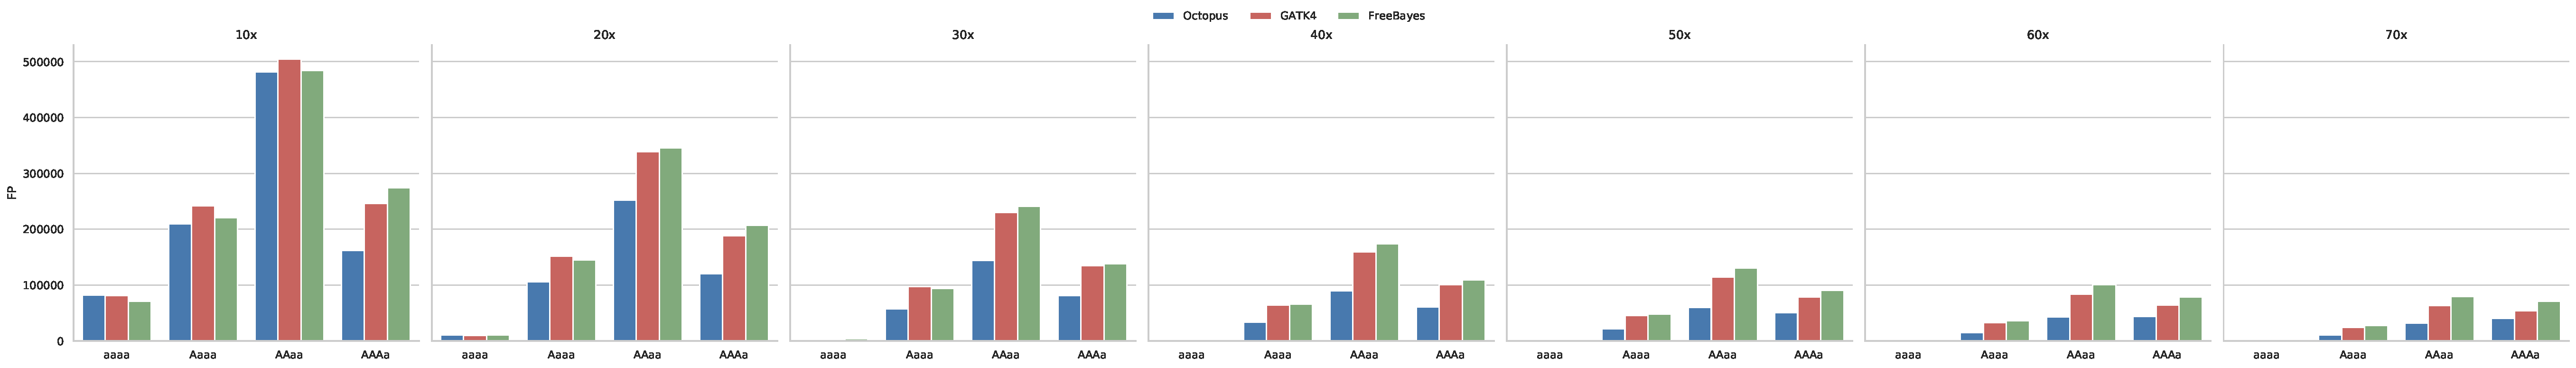
\includegraphics[width=\textwidth]{figures/tetraploid_gt_fp}
        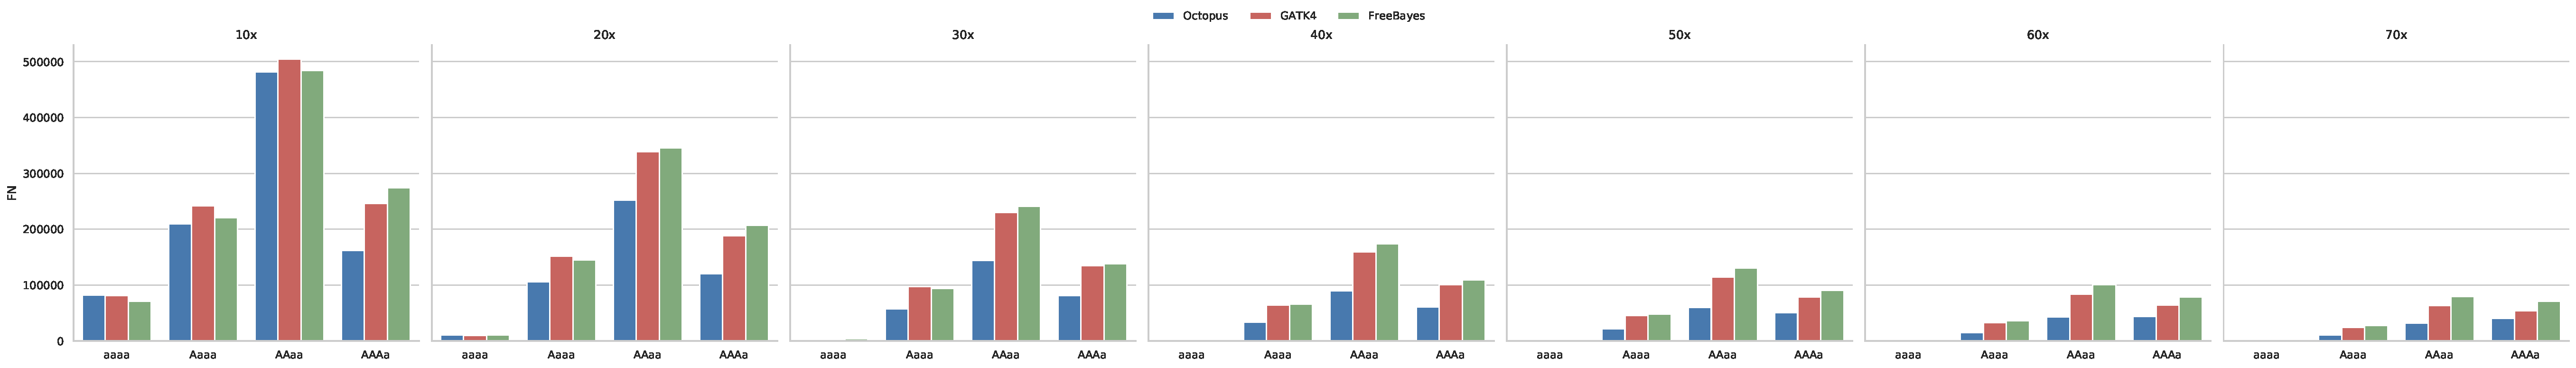
\includegraphics[width=\textwidth]{figures/tetraploid_gt_fn}
        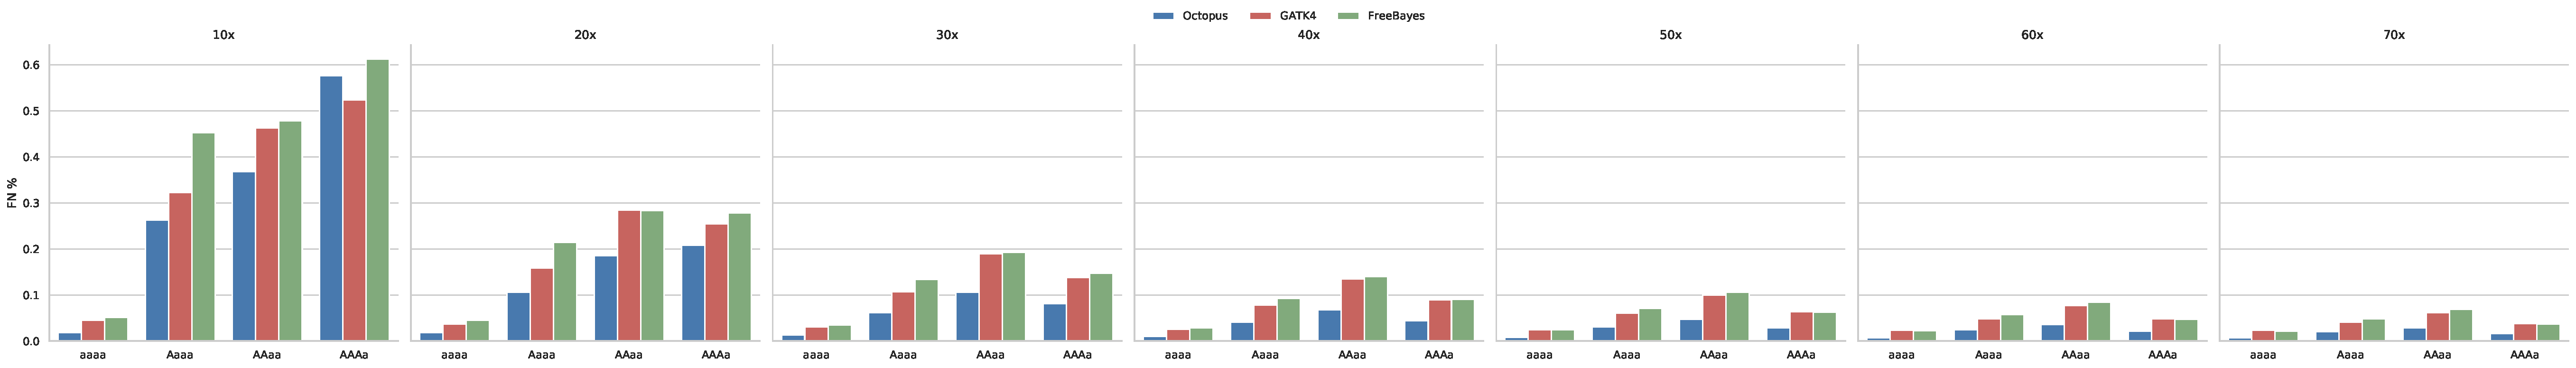
\includegraphics[width=\textwidth]{figures/tetraploid_gt_fn_perc}
        \label{fig:polyploid-genotyping-accuracy:tetraploid}
    \end{subfigure}
    \begin{subfigure}[b]{\textwidth}
        \caption{}
        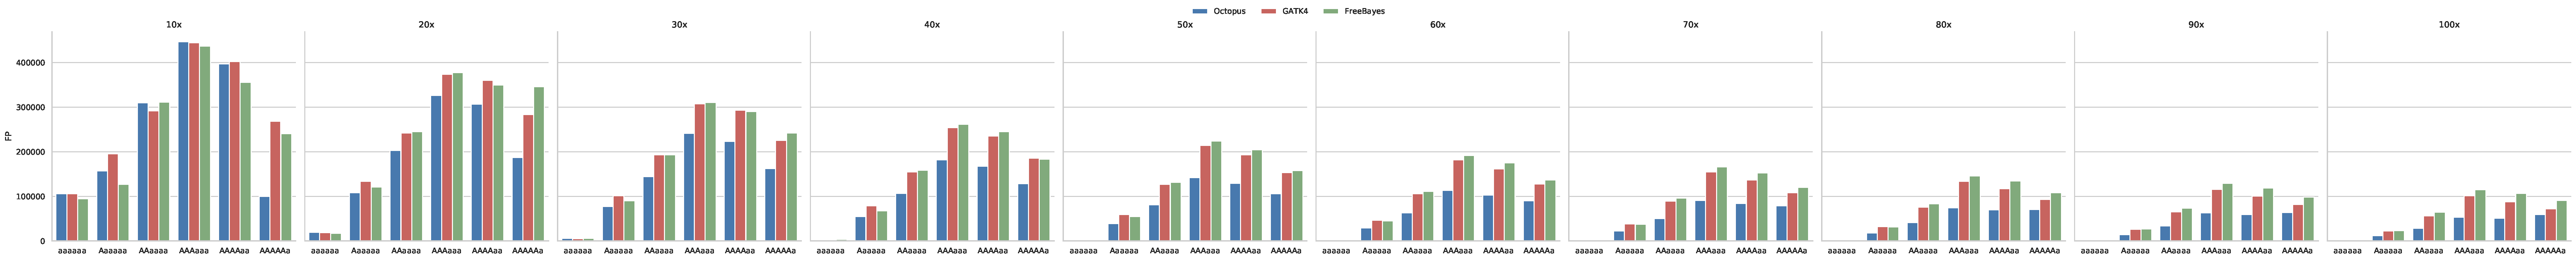
\includegraphics[width=\textwidth]{figures/hexaploid_gt_fp}
        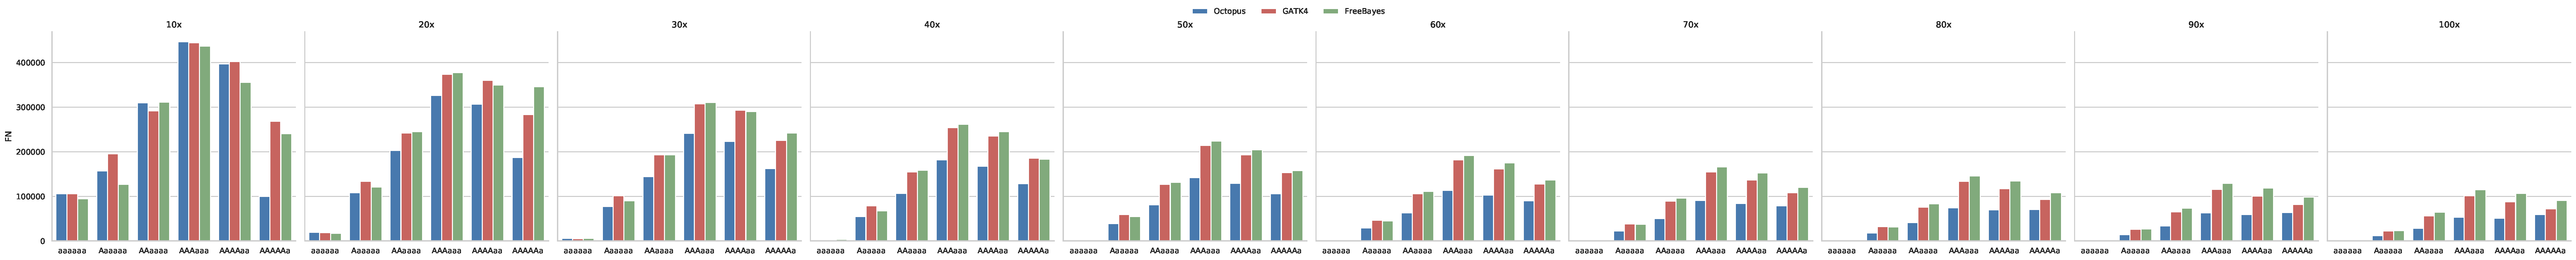
\includegraphics[width=\textwidth]{figures/hexaploid_gt_fn}
        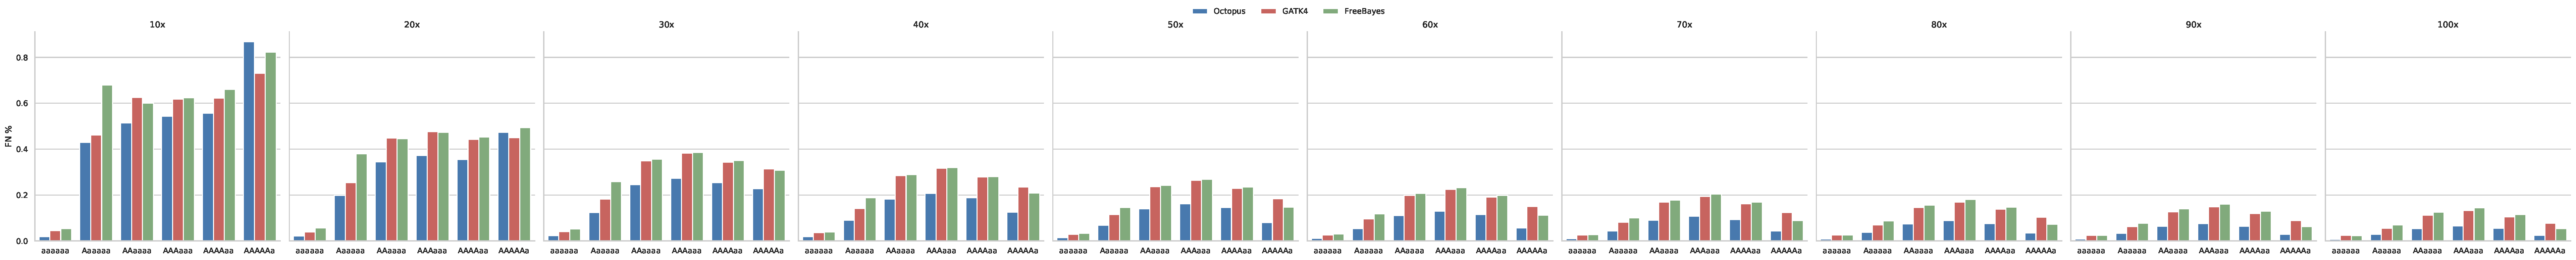
\includegraphics[width=\textwidth]{figures/hexaploid_gt_fn_perc}
        \label{fig:polyploid-genotyping-accuracy:hexaploid}
    \end{subfigure}
     \caption{\textbf{|\:Biallelic genotyping errors in synthetic polyploid samples.} \protect\subref{fig:polyploid-genotyping-accuracy:tetraploid} Tetraploid. \protect\subref{fig:polyploid-genotyping-accuracy:hexaploid} Hexaploid.}
    \label{supfig:polyploid_genotyping_accuracy}
\end{figure}

\clearpage

\begin{figure}[ht!]
    \centering
    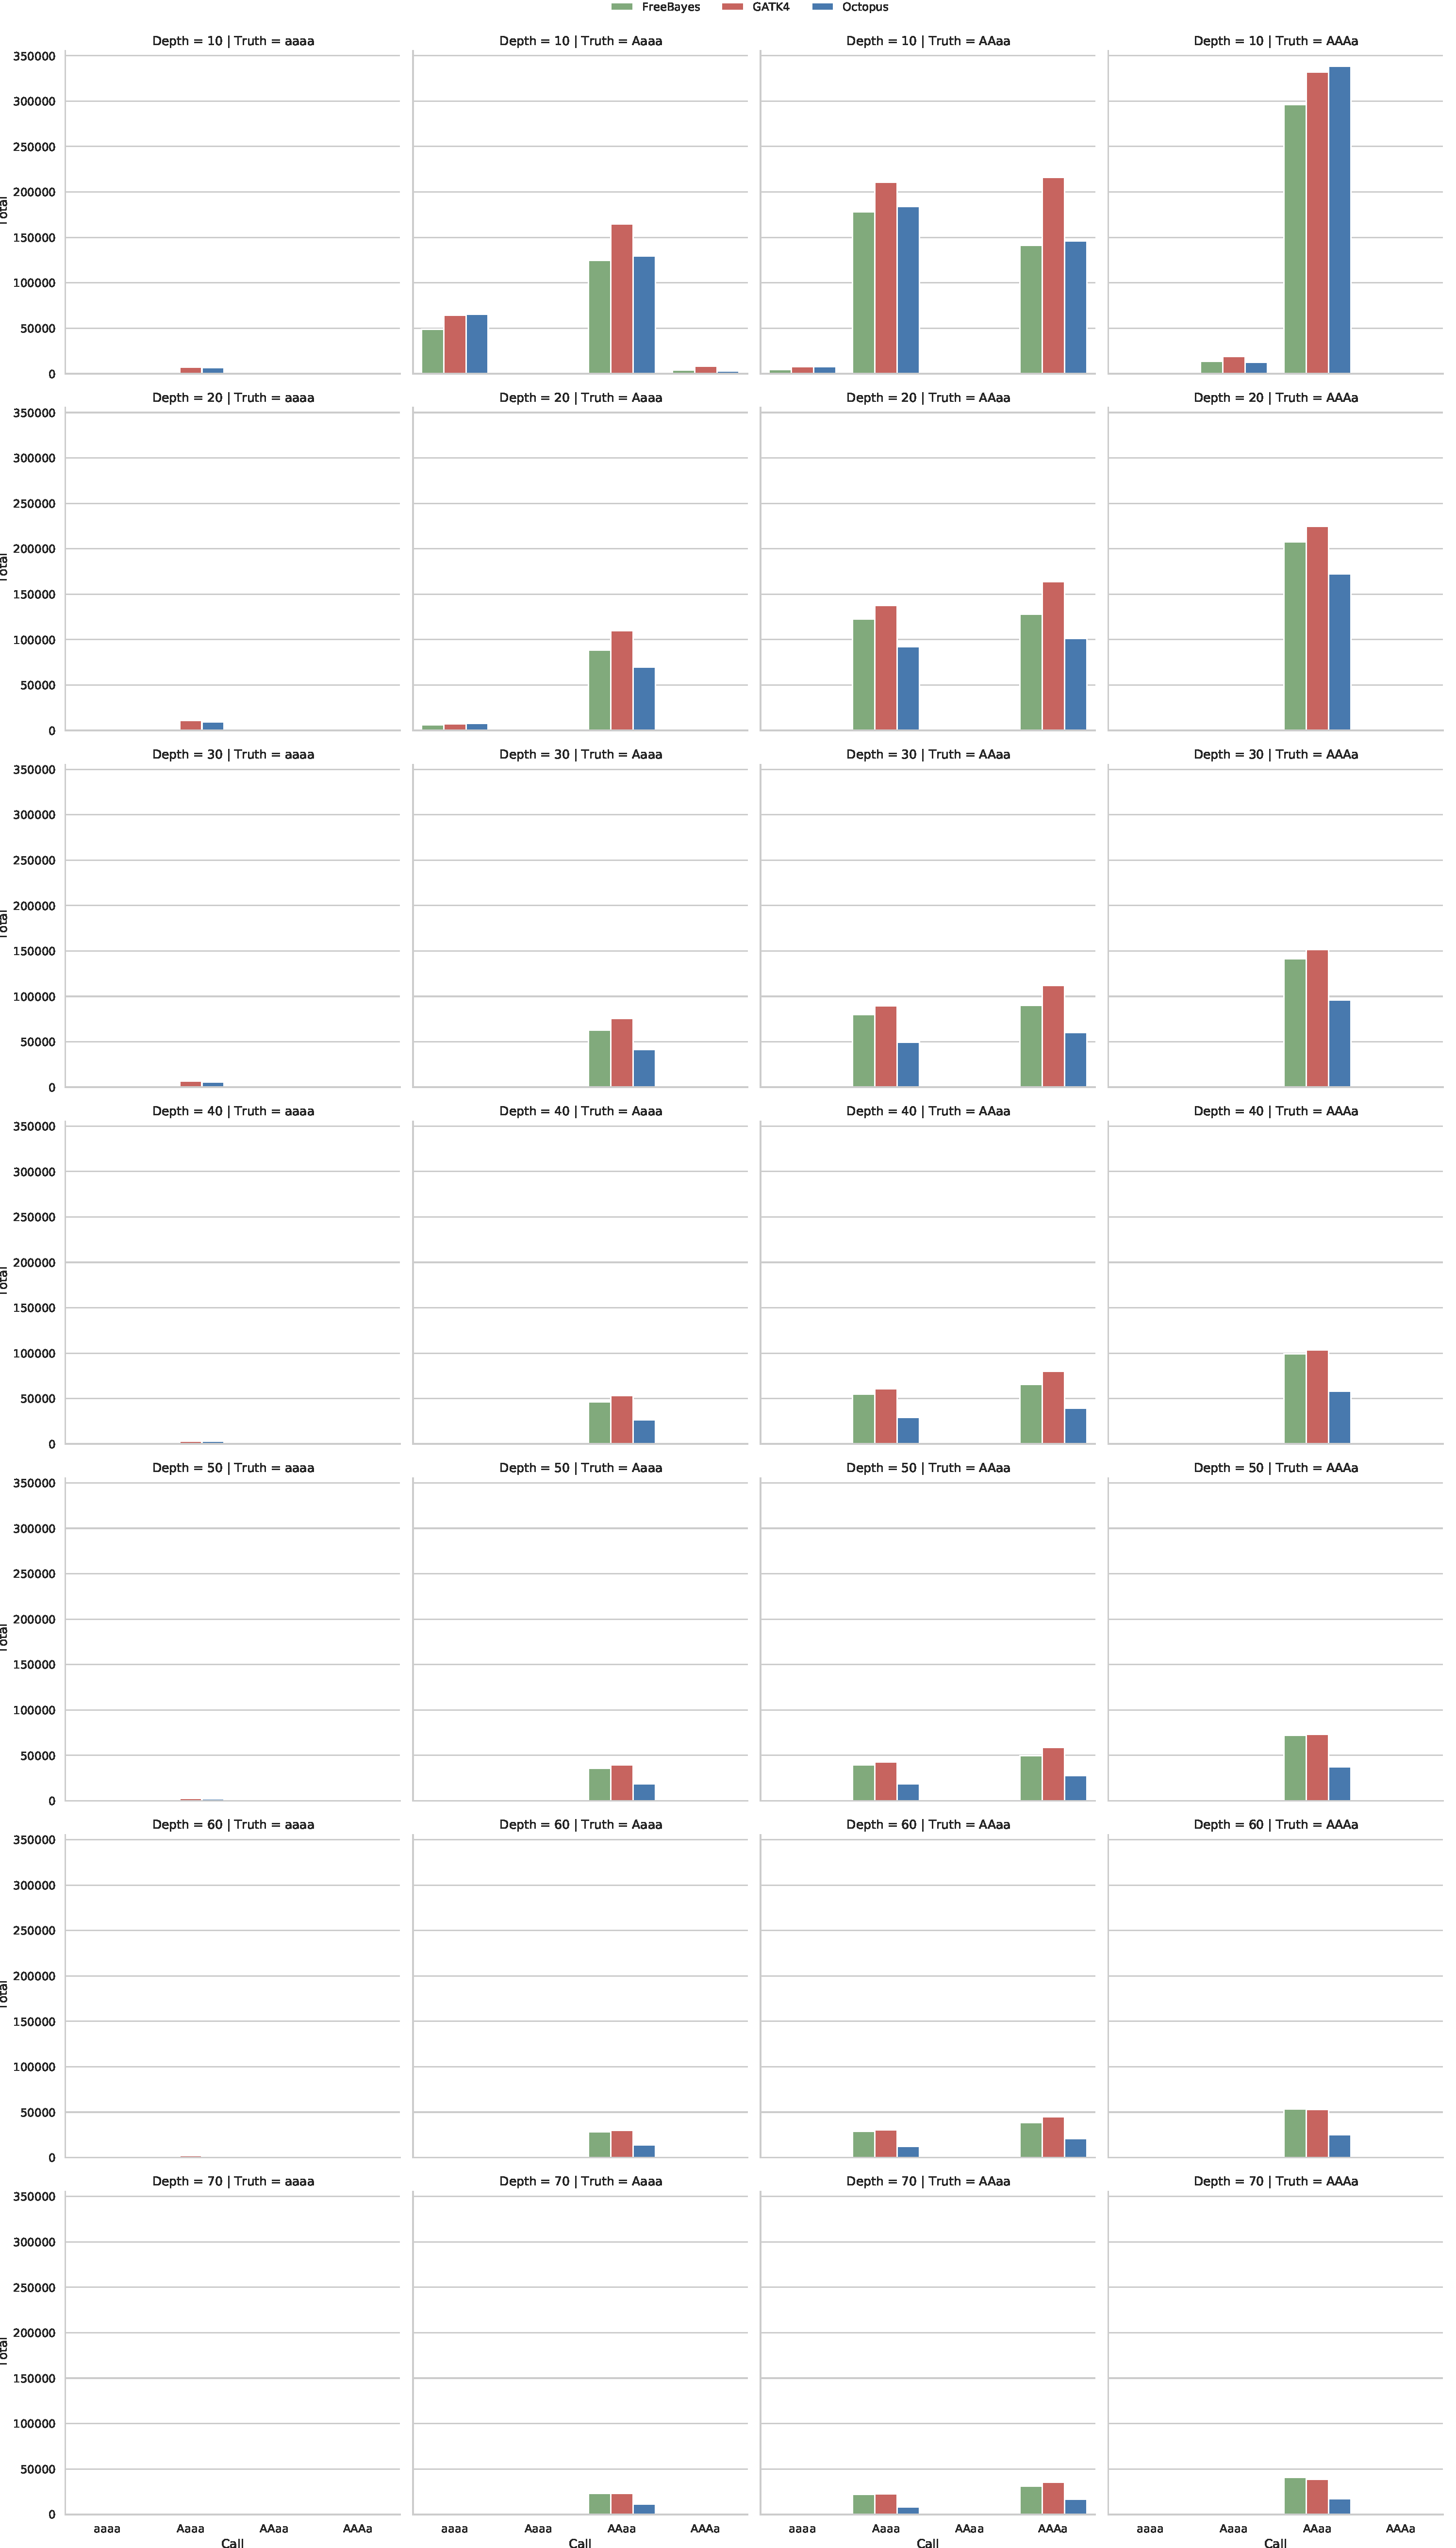
\includegraphics[height=0.95\textheight]{figures/tetraploid_biallelic_copy_errors}
    \caption{\textbf{|\:Biallelic copy number errors in synthetic tetraploid samples}.}
    \label{supfig:tetraploid_biallelic_copy_errors}
\end{figure}

\clearpage

\begin{figure}[ht!]
    \centering
    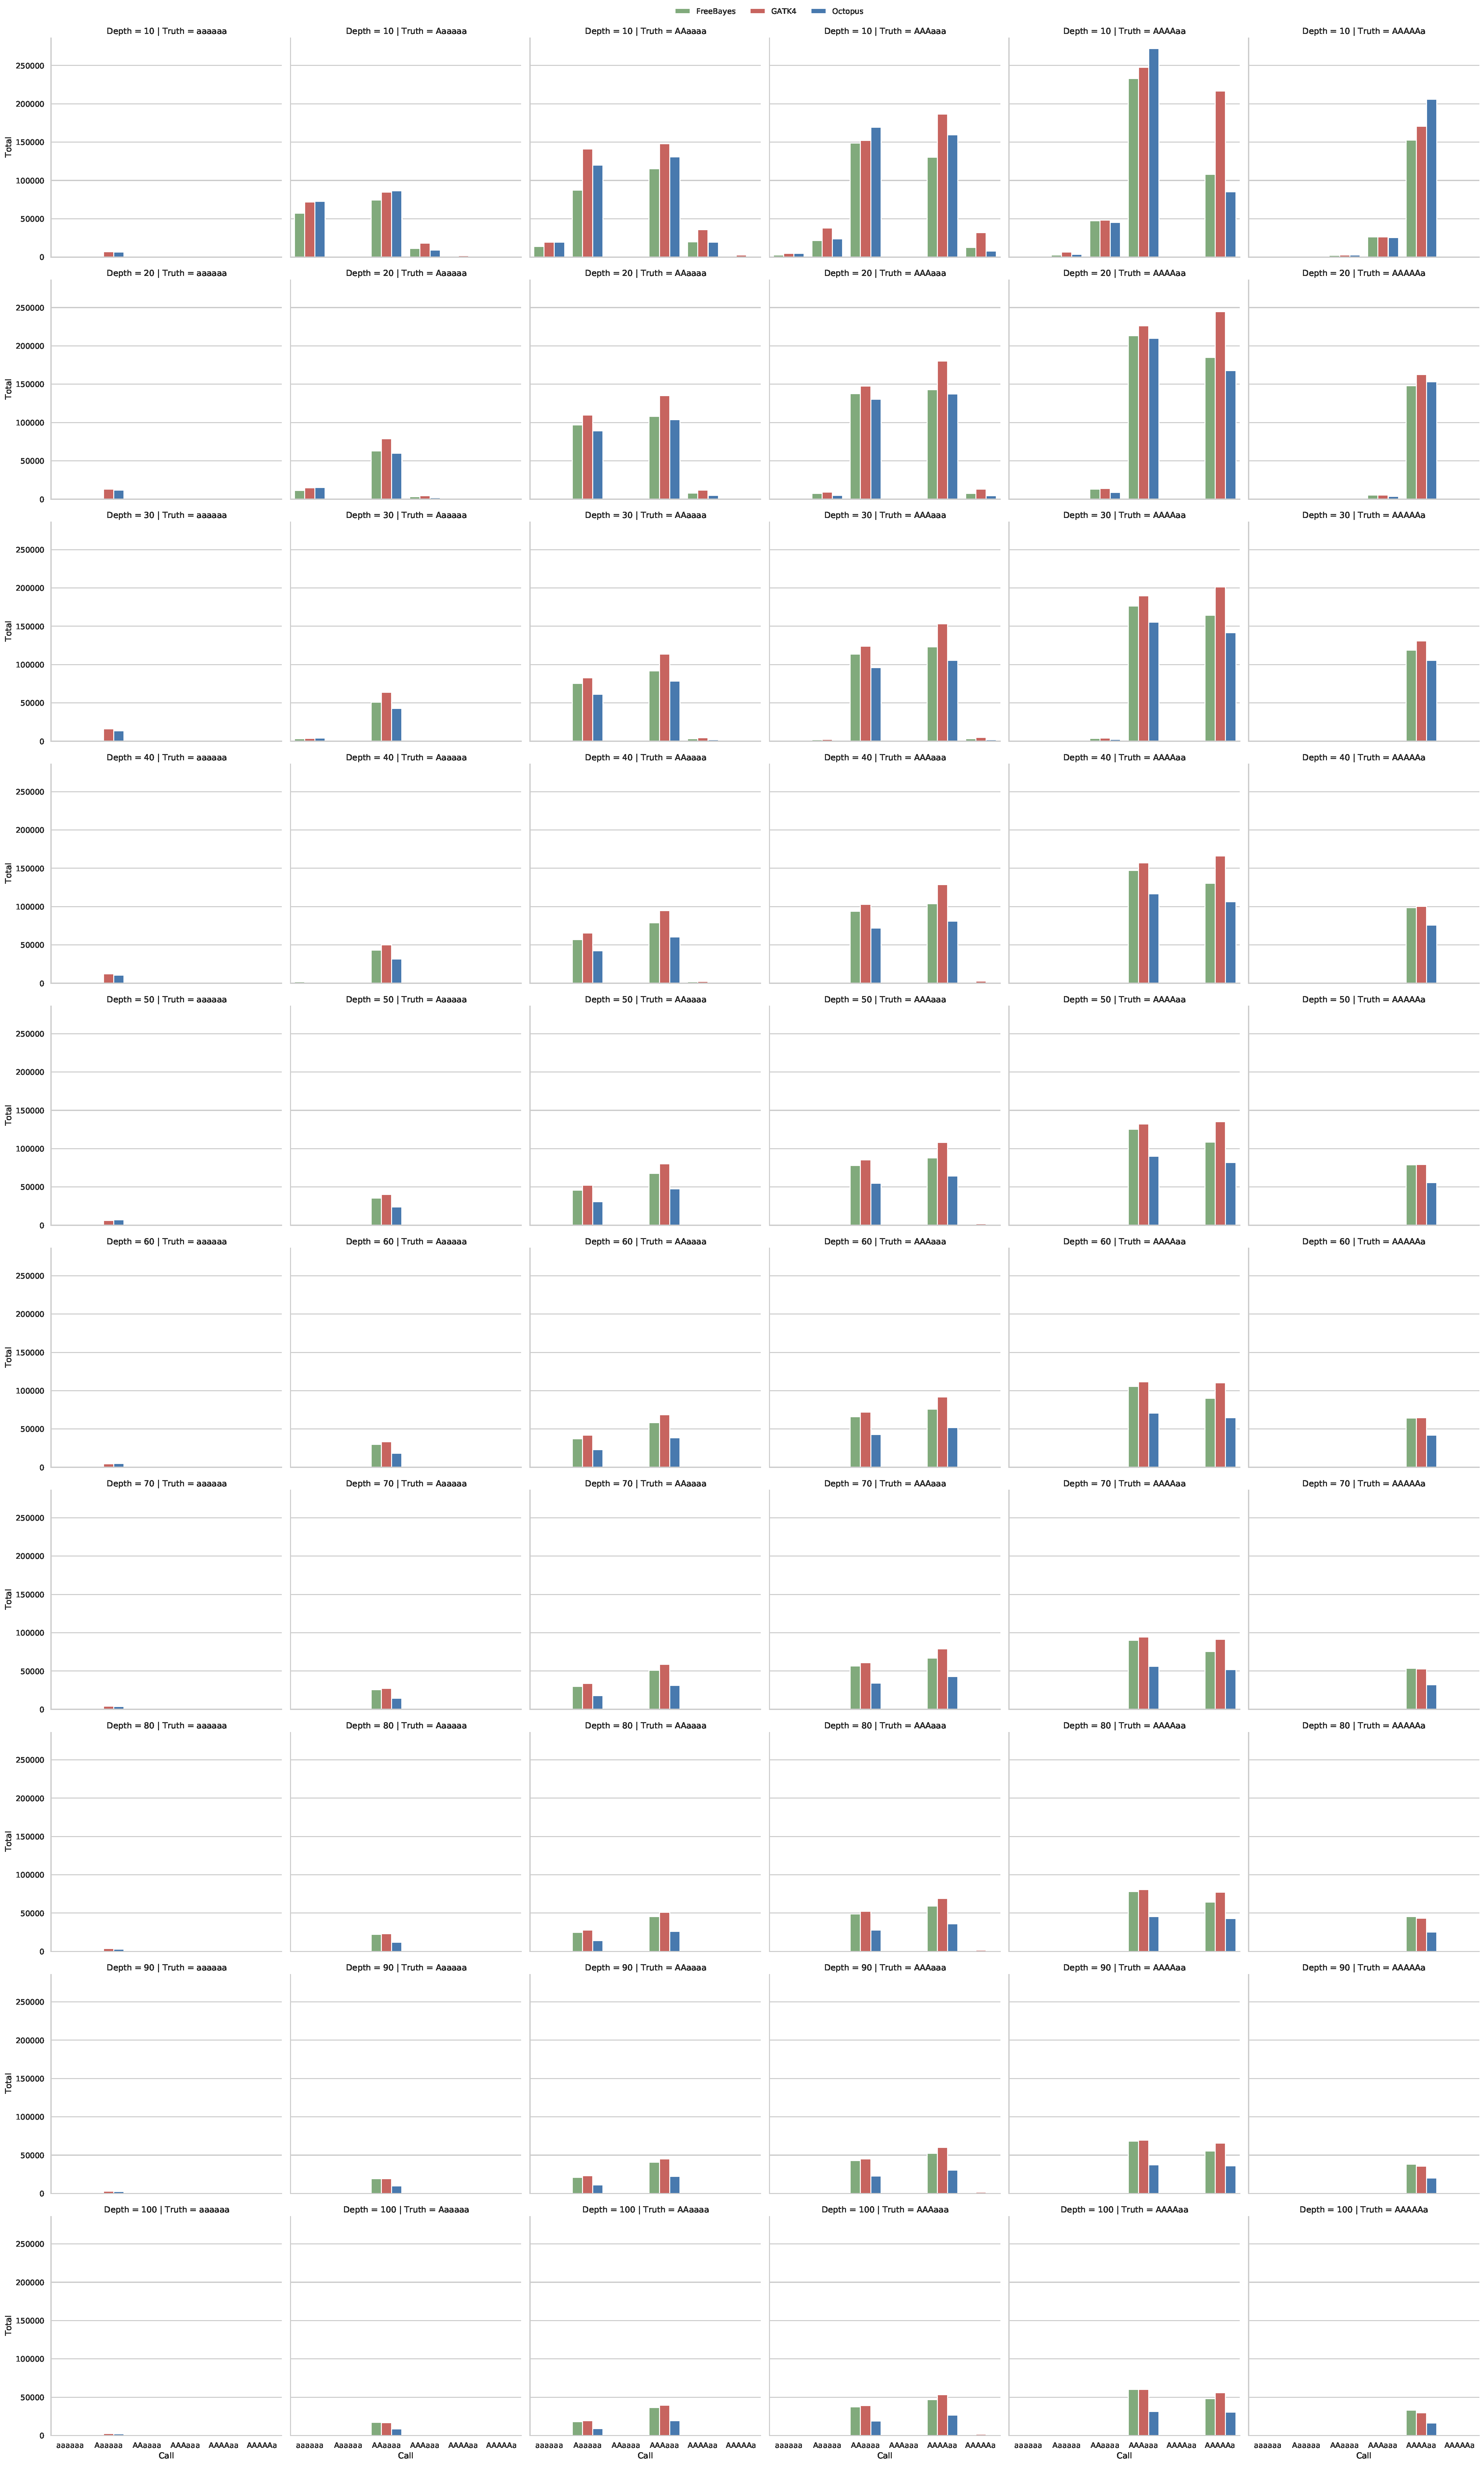
\includegraphics[height=0.95\textheight]{figures/hexaploid_biallelic_copy_errors}
    \caption{\textbf{|\:Biallelic copy number errors in synthetic hexaploid samples}.}
    \label{supfig:hexaploid_biallelic_copy_errors}
\end{figure}

\clearpage

\begin{figure}
    \centering
\captionsetup[subfigure]{position=top,labelfont=bf,textfont=normalfont,singlelinecheck=off,justification=raggedright}
    \begin{subfigure}[b]{\textwidth}
        \caption{}
        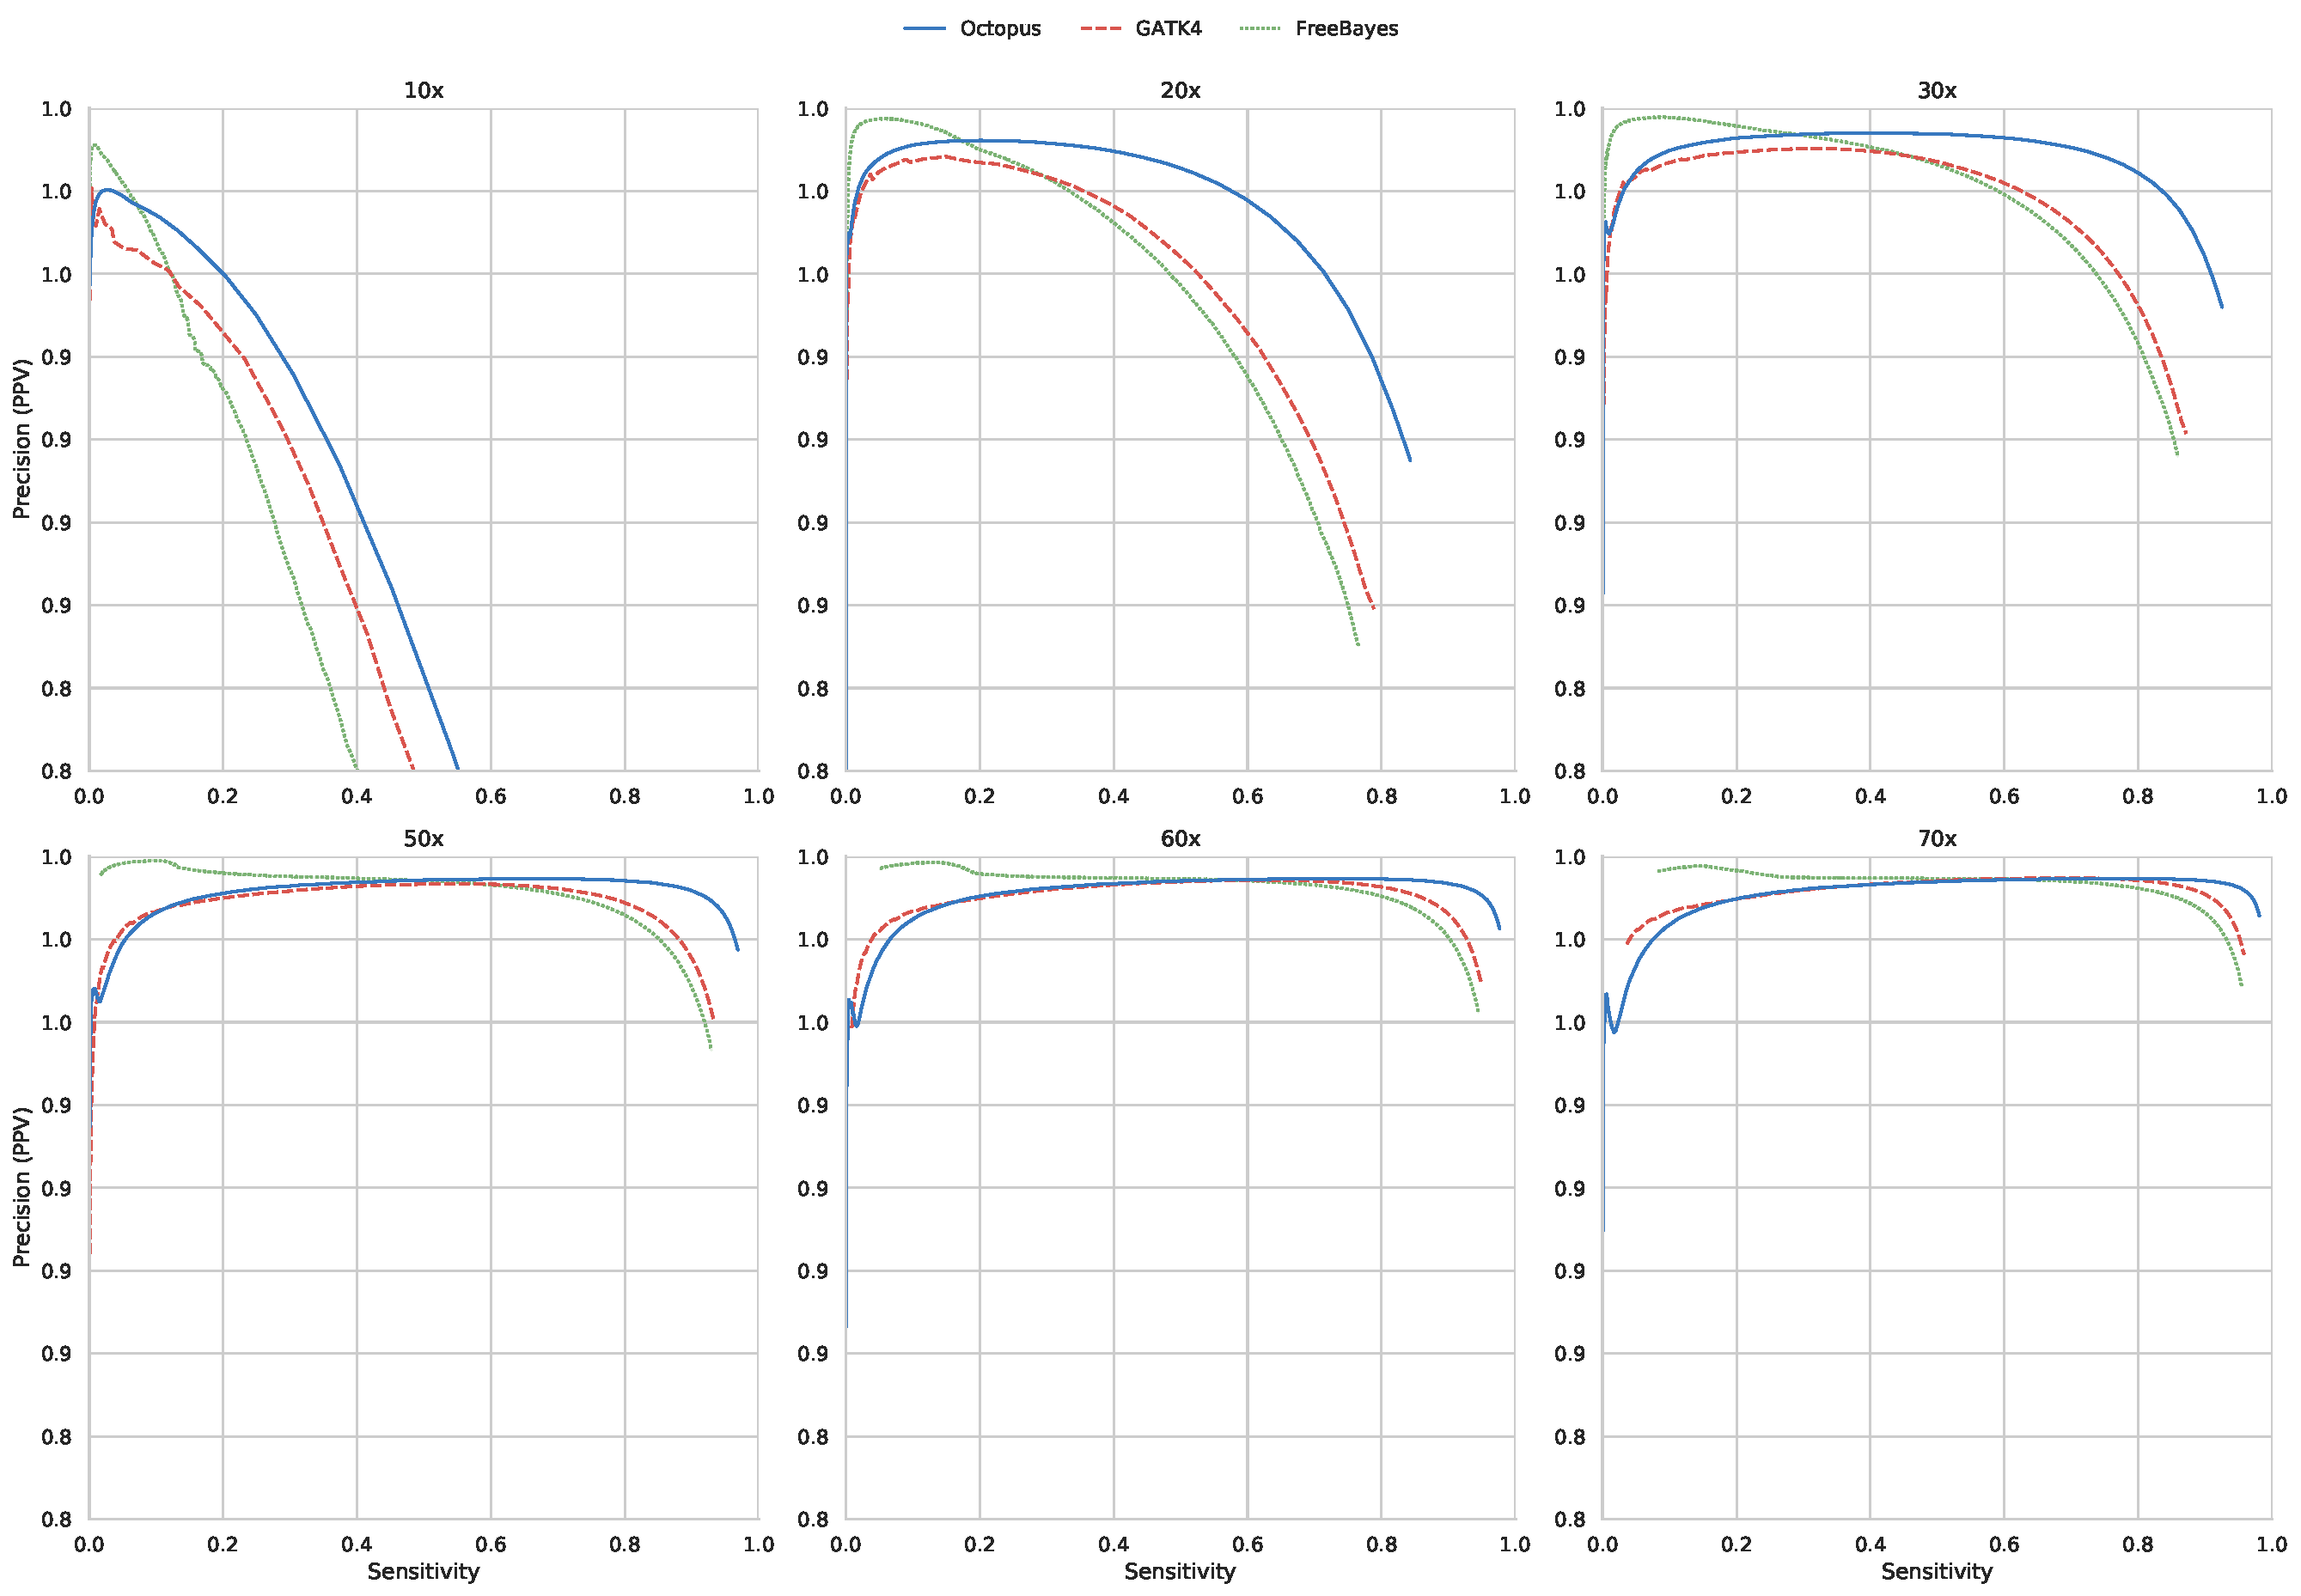
\includegraphics[width=\textwidth]{figures/synthetic-tetraploid-pr-curves}
        \label{fig:polyploid-genotyping-accuracy:tetraploid}
    \end{subfigure}
    \begin{subfigure}[b]{\textwidth}
        \caption{}
        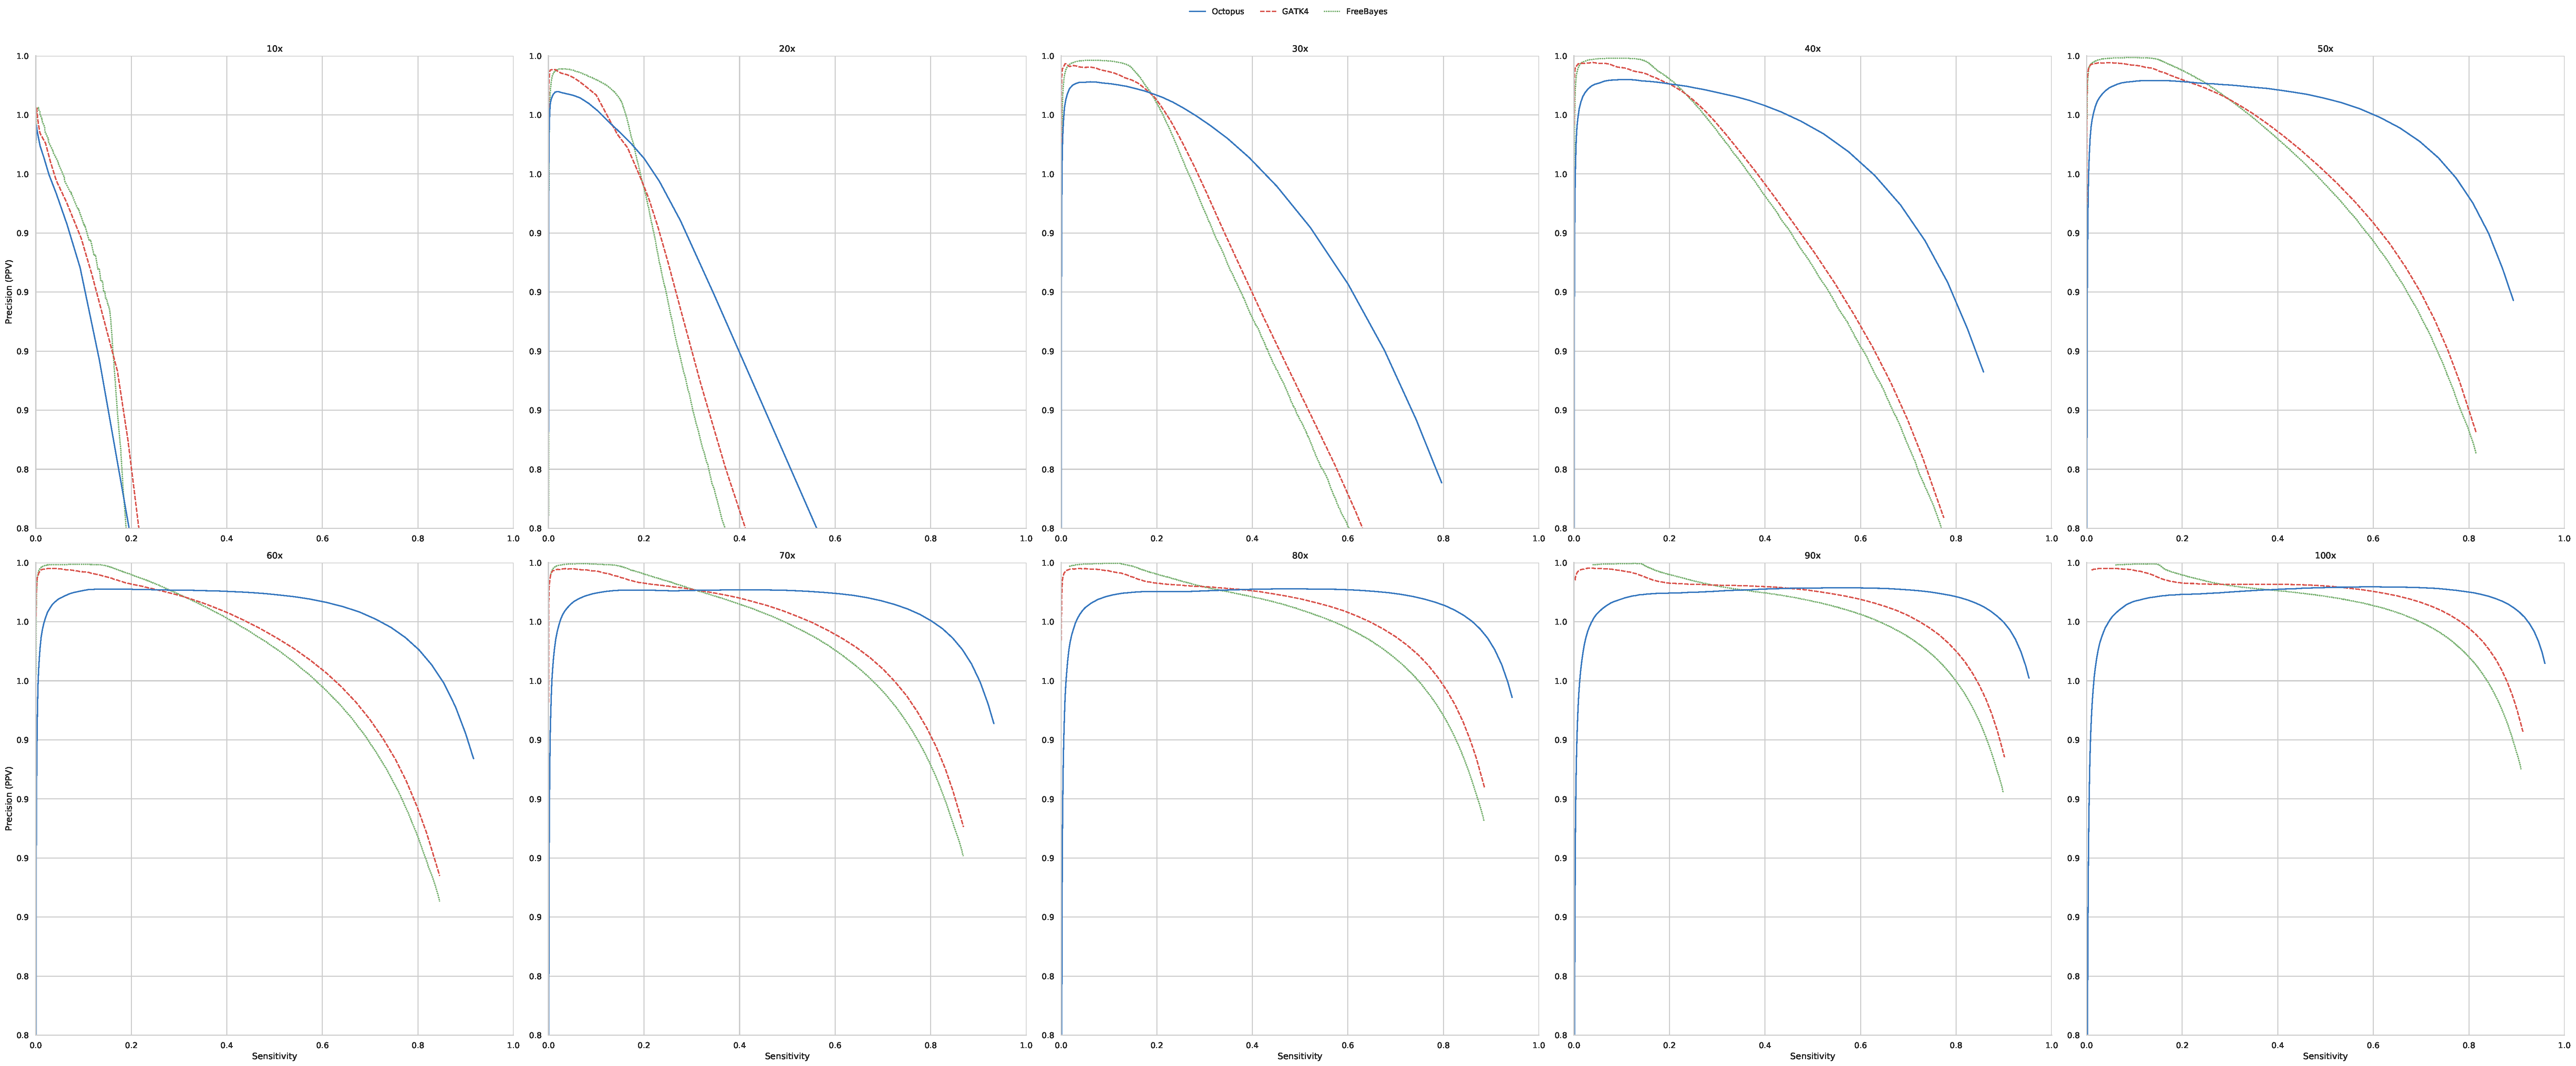
\includegraphics[width=\textwidth]{figures/synthetic-hexaploid-pr-curves}
        \label{fig:polyploid-genotyping-accuracy:hexaploid}
    \end{subfigure}
     \caption{\textbf{|\:Precision-recall curves for genotyping errors in synthetic polyploid samples.} GQ was used to generate curves for all samples. \protect\subref{fig:polyploid-genotyping-accuracy:tetraploid} Tetraploid. \protect\subref{fig:polyploid-genotyping-accuracy:hexaploid} Hexaploid.}
    \label{supfig:polyploid_prs}
\end{figure}

\clearpage

\begin{figure}[ht!]
    \centering
    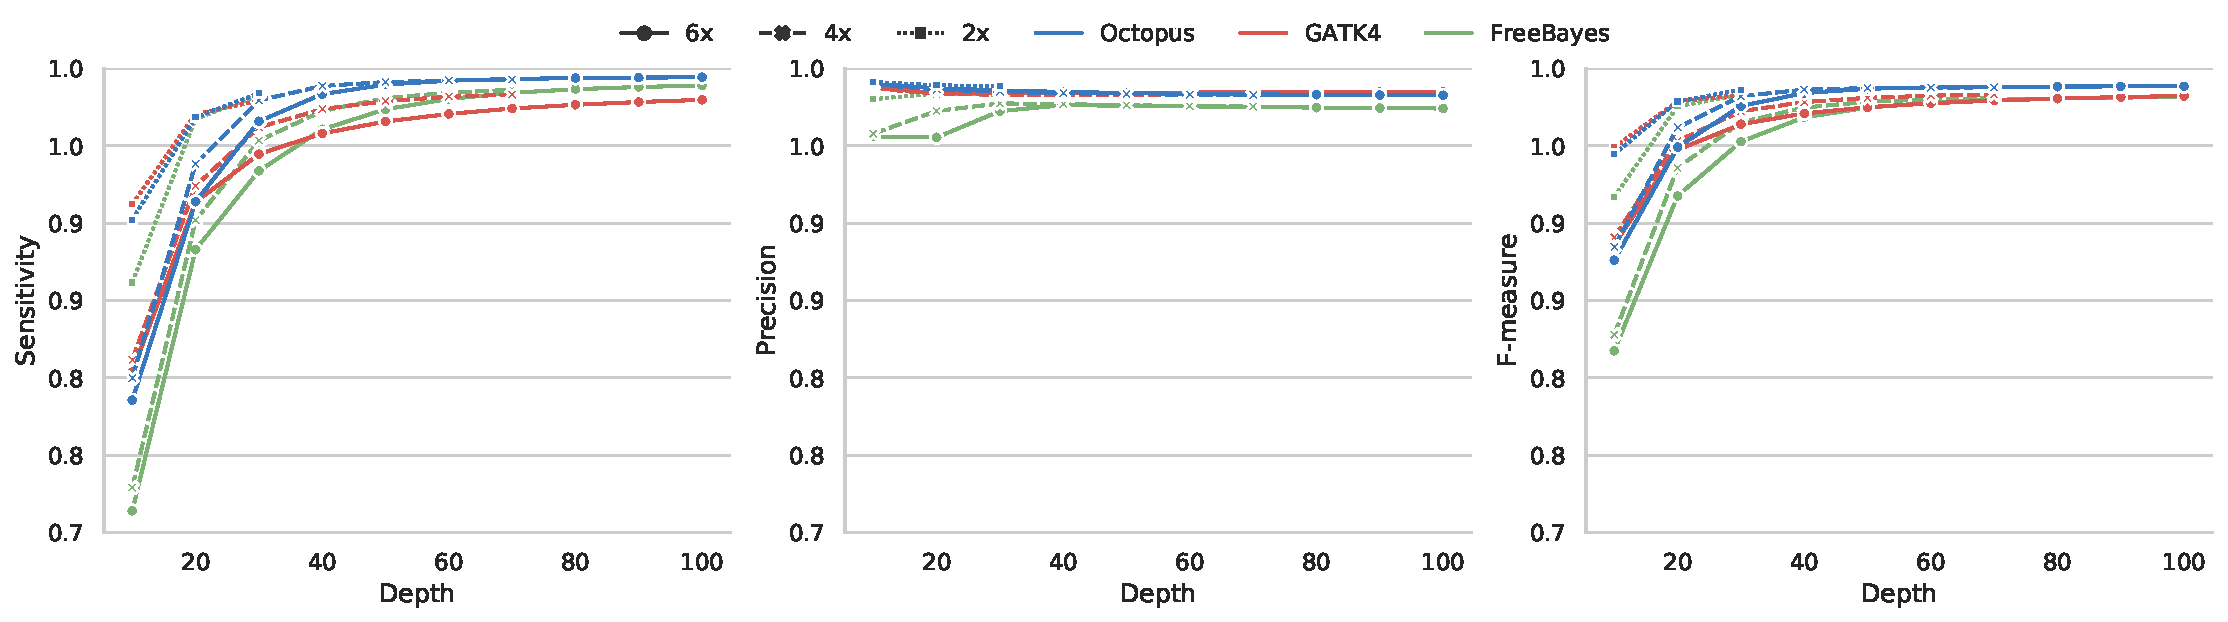
\includegraphics[width=\textwidth]{figures/accuracies-by-depth-alleles}
    \caption{\textbf{|\:Comparison of allele calling accuracies for diploid and synthetic polyploid datasets}.}
    \label{supfig:accuracies-by-depth-alleles}
\end{figure}

\clearpage

\begin{figure}[ht!]
    \centering
    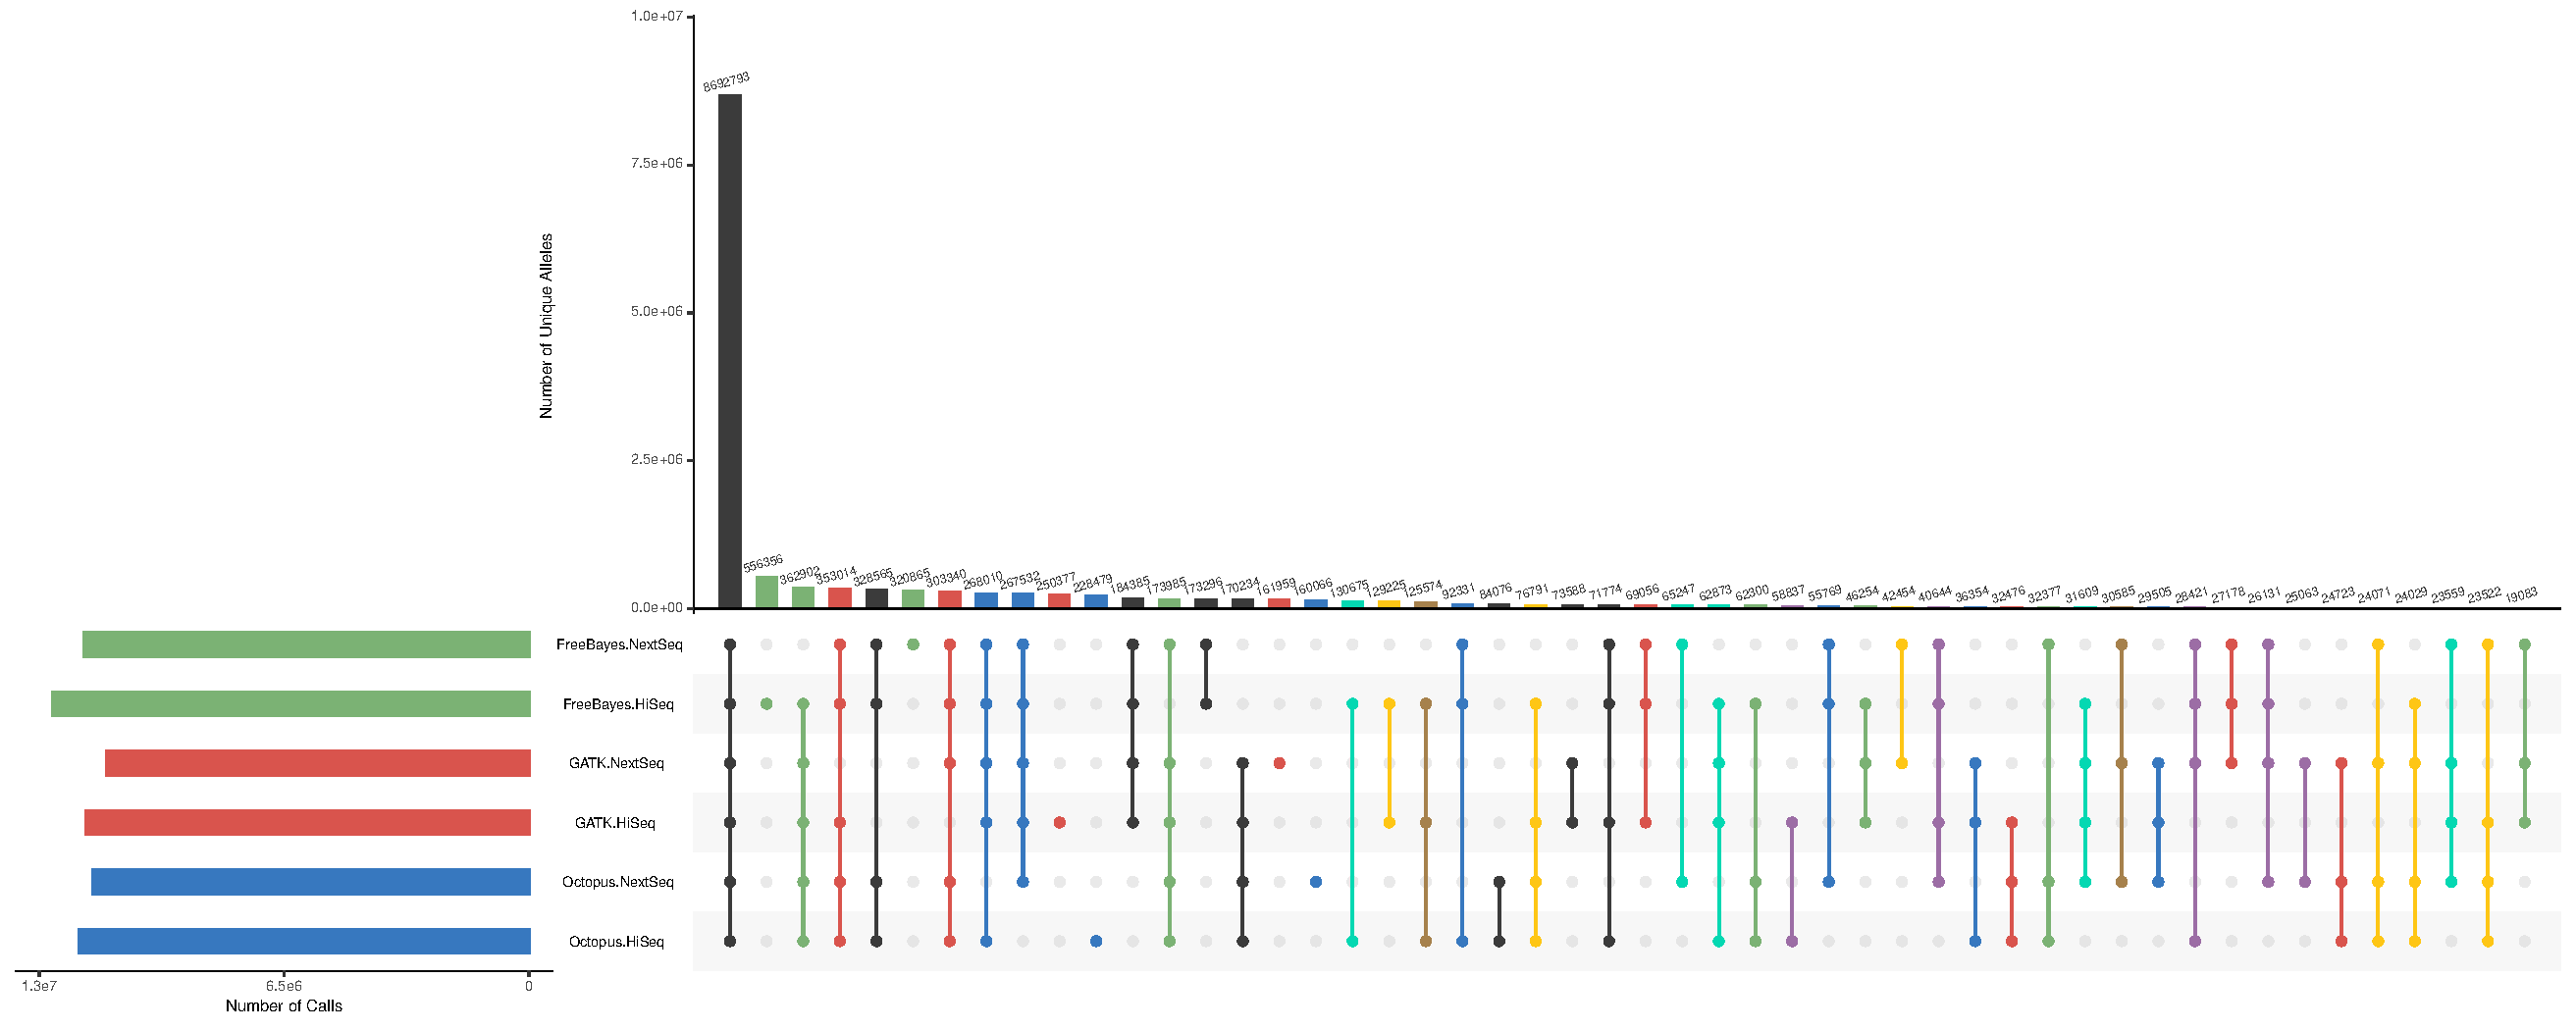
\includegraphics[width=\textwidth]{figures/banana_intersections_alleles}
    \caption{\textbf{|\:Comparison of alleles called in two Illumina datasets (HiSeq and NextSeq) of banana specimen by Octopus, GATK4, and FreeBayes}. UpSet plot shows callset intersections for each caller-dataset pair. The largest $50/63$ intersection sets are shown. Intersections are color coded by caller discordance between the two datasets: No discordances (black), Octopus (blue), GATK4 (red), FreeBayes (green), Octopus \& GATK4 (purple), Octopus \& FreeBayes (cyan), GATK4 \& FreeBayes (yellow), All (brown). The total number of unique alleles calls was \num[group-separator={,}]{14825250}.}
    \label{supfig:banana_intersections_alleles}
\end{figure}

%\section{Supplementary Note 1. Data and software}
%
%\begin{itemize}
%    \item seqtk (1.3)
%    \item samtools (1.11)
%    \item bcftools (1.11)
%    \item BWA (0.7.17)
%    \item pbmm2 (1.4.0)
%    \item bedtools (2.29.2)
%    \item RTG Tools (3.12)
%    \item Octopus
%    \item GATK4 (4.2.0.0)
%    \item FreeBayes (1.3.5)
%\end{itemize}

%\bibliographystyle{naturemag}
%\bibliography{supplementary}

\end{document} 
